\documentclass[12pt, xcolor=dvipsnames]{beamer}
%\usetheme{CambridgeUS}
\usetheme{Goettingen}
%\usecolortheme{dolphin}
\usecolortheme{rose}
%\useinnertheme{ default }
%	circles | default | inmargin |
%	rectangles | rounded}
%\useoutertheme{ shadow
%	default | infolines | miniframes |
%	shadow | sidebar | smoothbars |
%	smoothtree | split | tree
%}

\usepackage[utf8]{inputenc}
\usepackage[english]{babel}
\usepackage[T1]{fontenc}
\usepackage{amsmath}
\usepackage{amsfonts}
\usepackage{amssymb}
\usepackage{subfigure}
\usepackage{textpos}
\usepackage{bibgerm} 
\graphicspath{{./images/}}
%\setbeamerfont{page number in head/foot}{size=\large}
%\setbeamertemplate{footline}[page number]
\setbeamertemplate{footline}
{\begin{beamercolorbox}[sep=1ex]{author in head/foot}
		\rlap{}\hfill\hfill\llap{\large \insertframenumber}%
	\end{beamercolorbox}%
}
\setbeamercolor{sectioncolor}{fg=RoyalBlue, bg=white}

\AtBeginSection[]{
	\begin{frame}
		\vfill
		\centering
		\begin{beamercolorbox}[sep=8pt,center,shadow=true,rounded=true]{sectioncolor}
			\newline 
			\usebeamerfont{title}\insertsectionhead\par%
		\end{beamercolorbox}
		\vfill
	\end{frame}
}

\author[René Kremer]{\small René Kremer}
\title[An Overview and Comparison of PRIMEs and PERFoRMs Approach to take up the Challenge of Industrial Digitization]{An Overview and Comparison of PRIMEs and PERFoRMs Approach to take up the Challenge of Industrial Digitization}
\setbeamertemplate{navigation symbols}{} 
\titlegraphic{
	\begin{flushright}
	%\includegraphics[scale=0.1]{} 
	\end{flushright}}
\institute{Universität zu Lübeck} 
\date{26. Juni 2017} 

\begin{document}

\begin{frame}
	\titlepage
\end{frame}

% Magie für Templates oben rechts in der Ecke
\addtobeamertemplate{frametitle}{}{%
	\begin{textblock*}{100mm}(.85\textwidth,-1cm)
	\end{textblock*}}

%	\begin{frame}{Agenda}
%		\tableofcontents
%	\end{frame}

\section{Motivation}

\begin{frame}{Current Situation}
	\begin{itemize}
		\item Market globalization leads to higher demands of customers in terms of quality, cost and product customization
		\newline
		
		\item Industrial competitiveness also means shorter product lifecycles, increased product variety and shorter time-to-market
		\newline
		
		\item Companies need to face these changes with new manufacturing paradigms and business models
		\newline
		
		\item For production digitization and complete process integration, there is a need for concepts, techniques and technologies that will support it
	\end{itemize}
\end{frame}

\begin{frame}{Digitization leads to...}
	\begin{itemize}
		\item Resources becoming pluggable and smarter (communicating, cooperating, collaborating)
		\newline 
		
		\item the usage of the Cyber-Physical-Systems (CPS) paradigm
		\newline
		
		\item the need for a system to handle these heterogenous CPS
	\end{itemize}
\end{frame}

\begin{frame}{Emerging Problems}
	Manufacturers systems consist of:
	\begin{itemize}
		\item Mostly centralized legacy systems and control mechanisms
		\newline
		
		\item Heterogenous components
	\end{itemize}
\end{frame}

\begin{frame}{Approach for the Future}
	\begin{itemize}
		\item Distributed and agile systems
		\newline
		
		\item System components functionality decoupled as services
		\newline
		
		$\Rrightarrow$ service-based architectures like the Service-oriented Architecture (SoA)
		\newline
		
		\item Seamless vertical and horizontal system integration
	\end{itemize}
\end{frame}

\begin{frame}{State of the Art Methodologies}
	\begin{itemize}
		\item Multi-Agent Systems (MAS)
		\newline
		
		\item Plug and Produce Technology
		\newline
		
		\item Service-oriented Architecture
		\newline
		
		\item Cloud Technology
	\end{itemize}
\end{frame}

\section[PRIME] {PRIME}

\subsection{What is PRIME}
\begin{frame}{What is PRIME I}
	\begin{itemize}
		\item Result of the EU funded FP7 PRIME project (2007 - 2013)
		\newline
	 
		\item Architecture using a hybrid structure integrating a MAS with traditional automation equipment
		\newline

	\end{itemize}
\end{frame}

\begin{frame}{What is PRIME II}
	\begin{itemize}
		\item MAS handles reconfiguration of the productions control system
		\newline
				
		$\Rrightarrow$ Agent technology might lead to time processing issues of communication and process control
		\newline
		
		\item Productions control system and MAS operate independently
		\newline
		
		$\Rrightarrow$ lessens burdens of MAS and increase flexibility of the overall system
	\end{itemize}
\end{frame}

\subsection{Architecture}
\begin{frame}{Architecture}
	\begin{figure}
		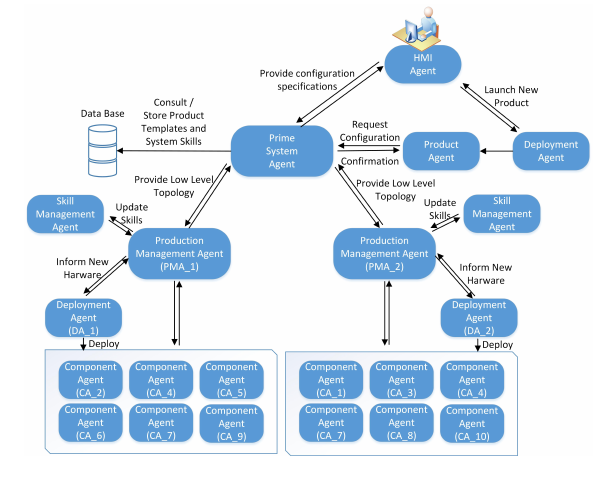
\includegraphics[scale=0.435]{PRIME/PRIME-Architecture}
		\caption{PRIME-Architecture \cite{Hybrid}}
	\end{figure}
\end{frame}

\begin{frame}{Production Management Agent Tree}
	\begin{figure}
		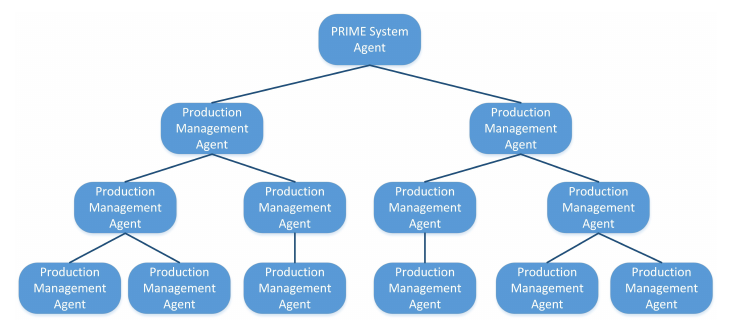
\includegraphics[scale=0.385]{PRIME/Production-Management-Agent-Tree}
		\caption{Production-Management-Agent-Tree \cite{Hybrid}}
	\end{figure}
\end{frame}

\section{PERFoRM}
\subsection{What is PERFoRM}
\begin{frame}{What is PERFoRM I}
	\begin{exampleblock}{PERFoRM}
		The EU HORIZON 2020 project PERFoRM (Production harmonizEd Reconfiguration of Flexible Robots and Machinery) is aiming at the \textbf{conceptual transformation} of \emph{existing} production systems towards \textbf{agile}, \textbf{networked plug-and-produce production systems} in order to achieve a \emph{flexible manufacturing environment} based on f\textbf{ast reconfiguration} of machinery and robots as response to operational or business events. \cite{Harmonized}
	\end{exampleblock}
\end{frame}

\begin{frame}{What is PERFoRM II}
	Architecture (currently researched and specified) to support the production digitalization by providing:
	\newline 
	\begin{itemize}
		\item service-orientation to expose system functionalities as services
		\newline
		
		\item a middleware as a common platform for information exchange
		\newline
		
		\item a common language for standard interfaces
		\newline  
	\end{itemize}
\end{frame}

\begin{frame}{What is PERFoRM III}
	Further support by providing:
	\newline
	\begin{itemize}
		\item technology adapters to integrate legacy systems
		\newline
		
		\item a Human-Machine-Interface (HMI) to allow the human to interact with the system and drive its flexibility
	\end{itemize}
\end{frame}

\subsection{Architecture}

\begin{frame}{PERFoRM Architecture - Overview}
	\begin{figure}
		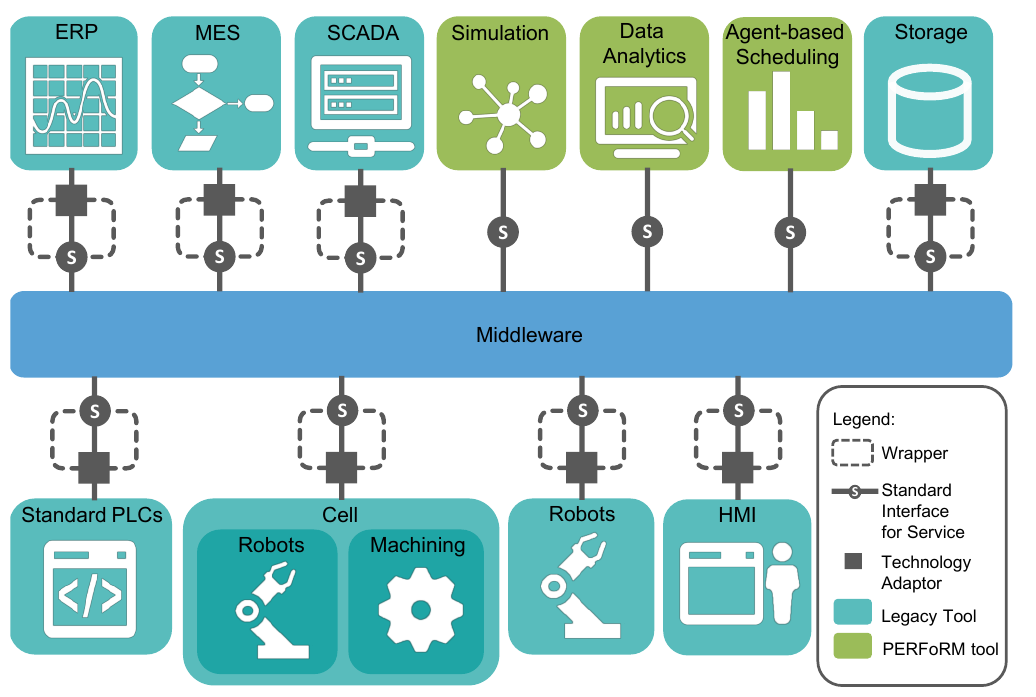
\includegraphics[scale=0.25]{Specification-PERFoRM/PERFoRM-Architecture}
		\caption{PERFoRM Architecture \cite{Perform}}
	\end{figure}
\end{frame}

\section{Comparison}

\subsection{Seamless reconfiguration}
\begin{frame}{Seamless reconfiguration I}
	\begin{itemize}
		\item PRIME shows a good solution in terms of reconfiguration time
		\newline
		
		\item PSA as bottleneck has yet to be tested
		\newline
		
		\item PSA and PMA are single points of failure
		\newline
		
		$\Rrightarrow$ Backup plan needed!
		\newline
		
		First ideas: Heartbeat algorithm, reboot of dead agents, remapping of children of dead PMAs
	\end{itemize}
\end{frame}

\begin{frame}{Seamless reconfiguration II}
	PERFoRM recognizes the need for seamless reconfiguration and...
	\newline 
	
	\begin{itemize}
		\item suggests MAS or SoA for this issue
		\newline
		
		\item assumes that components will be enriched with Artifical Intelligence methods
		\newline
	\end{itemize}
\end{frame}

\begin{frame}{Seamless reconfiguration III}
	PERFoRM might adopt PRIMEs approach to fulfill the requirement of seamless reconfiguration
	\newline
		
	\begin{itemize}
		\item where will PRIMEs MAS find its place?
		\newline
			
	\end{itemize}
	$\Rrightarrow$ Middleware? As a PERFoRM Tool? A combination of both?
\end{frame}

\subsection{Integration of existing systems}

\begin{frame}{Integration of existing systems I}
	PRIMEs Component Agents handle
	\newline
	
	\begin{itemize}
		\item communication
		\newline
		
		\item parametrization
		\newline
		
		\item configuration of physical components
		\newline
		
	\end{itemize}
	
	PRIME leaves no hint about legacy system integration
\end{frame}

\begin{frame}{Integration of existing systems II}
	\begin{itemize}
		\item PERFoRM specifies standard interfaces and technology adapters for integrating software and hardware
		\newline
		
		\item Specification demand common data models
		\newline
		
		\item Middleware handles communication
		\newline
		
		$\Rrightarrow$ single point of failure (as PSA/PMA in PRIME)
	\end{itemize}
\end{frame}

\begin{frame}{Integration of existing systems III}
	\begin{itemize}
		\item MAS and PRIMEs approach will benefit from PERFoRMs communication infrastructure
		\newline
		
		\item PRIME fulfills the requirement of seamless reconfiguration mentioned by PERFoRMs specification
		\newline
		
		\item Skills of PRIME can be described as services in PERFoRM for a SoA approach
		\newline
		
	\end{itemize}
\end{frame}

\subsection{Conclusion}

\begin{frame}{Conclusion}
	\begin{itemize}
		\item PRIME and PERFoRM tackle other challenges of the digitization
		\newline
		
		\item Integrating PRIMEs reconfiguration aspect in PERFoRM might lead to an important and strong backbone
		\newline
		
		\item Reevaluation necessary once PERFoRMs full specification is clear and an implementation is presented
		\newline
		
	\end{itemize}
\end{frame}

\section{References}
\begin{frame}[allowframebreaks]{Outline}
	\frametitle{Reference}
	\bibliographystyle{abbrv}
	\bibliography{./bib/presentation}
	\nocite{Perform}
	\nocite{DataMining}
	\nocite{FactoryOfTheFuture}
	\nocite{Harmonized}
	\nocite{Hybrid}
	\nocite{ModularProduction}
	\nocite{PlugProduce}
	\nocite{HighlyFlexible}
\end{frame}

\end{document}